\newpage
\section{Contexto da Instituição e do Curso}

\subsection{Contexto da Instituição}

\subsubsection{Dados da mantenedora}

% Please add the following required packages to your document preamble:
% \usepackage[table,xcdraw]{xcolor}
% If you use beamer only pass "xcolor=table" option, i.e. \documentclass[xcolor=table]{beamer}
\begin{table}[h]
\begin{tabular}{|
>{\columncolor[HTML]{C0C0C0}}l |
>{\columncolor[HTML]{FFFFFF}}l |
>{\columncolor[HTML]{FFFFFF}}l
>{\columncolor[HTML]{FFFFFF}}l
>{\columncolor[HTML]{FFFFFF}}l
>{\columncolor[HTML]{FFFFFF}}l |
>{\columncolor[HTML]{FFFFFF}}l |
>{\columncolor[HTML]{FFFFFF}}l |}
\hline
Mantenedora & \multicolumn{7}{l|}{\cellcolor[HTML]{FFFFFF}\begin{tabular}[c]{@{}l@{}}Instituto Federal de Educação, Ciência e Tecnologia\\ da Paraíba - CNPJ - 10.783.898/0001-75\\ Pessoa Jurídica de Direito Público – Federal\end{tabular}}                                                            \\ \hline
Endereço    & \multicolumn{5}{l|}{\cellcolor[HTML]{FFFFFF}Avenida Primeiro de Maio}                                                                                                                                                                   & \cellcolor[HTML]{C0C0C0}Número:       & 720       \\ \hline
Bairro      & Jaguaribe                                      & \cellcolor[HTML]{C0C0C0}Cidade:                                     & João Pessoa                                              & \cellcolor[HTML]{C0C0C0}CEP:        & 58015-430       & \cellcolor[HTML]{C0C0C0}UF:           & PB        \\ \cline{1-3} \cline{5-8}
Telefone:   & \multicolumn{2}{l|}{\cellcolor[HTML]{FFFFFF}\begin{tabular}[c]{@{}l@{}}(83) 3208 3000\\ (83) 3208 3004\end{tabular}} & \multicolumn{1}{l|}{\cellcolor[HTML]{C0C0C0}Fax:}        & \multicolumn{4}{l|}{\cellcolor[HTML]{FFFFFF}(83) 3208 3088}                                               \\ \hline
E-mail:     & \multicolumn{7}{l|}{\cellcolor[HTML]{FFFFFF}ifpb@ifpb.edu.br}                                                                                                                                                                                                                               \\ \hline
Site:       & \multicolumn{7}{l|}{\cellcolor[HTML]{FFFFFF}www.ifpb.edu.br}                                                                                                                                                                                                                                \\ \hline
\end{tabular}
\end{table}

%colocar sub

\subsubsection{Dados da mantida}

% Please add the following required packages to your document preamble:
% \usepackage[table,xcdraw]{xcolor}
% If you use beamer only pass "xcolor=table" option, i.e. \documentclass[xcolor=table]{beamer}
\begin{table}[h]
\begin{tabular}{|
>{\columncolor[HTML]{C0C0C0}}l |
>{\columncolor[HTML]{FFFFFF}}l |
>{\columncolor[HTML]{FFFFFF}}l
>{\columncolor[HTML]{FFFFFF}}l
>{\columncolor[HTML]{FFFFFF}}l
>{\columncolor[HTML]{FFFFFF}}l |
>{\columncolor[HTML]{FFFFFF}}l |
>{\columncolor[HTML]{FFFFFF}}l |}
\hline
Mantida   & \multicolumn{7}{l|}{\cellcolor[HTML]{FFFFFF}\begin{tabular}[c]{@{}l@{}}IFPB - Campus Guarabira\end{tabular}}                                                                                       \\ \hline
Endereço  & \multicolumn{5}{l|}{\cellcolor[HTML]{FFFFFF}Rua José Américo}                                                                                              & \cellcolor[HTML]{C0C0C0}Número: & s/n \\ \hline
Bairro    & Bairro Nordeste I     & \cellcolor[HTML]{C0C0C0}Cidade:     & Guarabira                                         & \cellcolor[HTML]{C0C0C0}CEP: & 58200-000 & \cellcolor[HTML]{C0C0C0}UF:     & PB  \\ \cline{1-3} \cline{5-8}
Telefone: & \multicolumn{2}{l|}{\cellcolor[HTML]{FFFFFF}(83) 9188 0604} & \multicolumn{1}{l|}{\cellcolor[HTML]{C0C0C0}Fax:} & \multicolumn{4}{l|}{\cellcolor[HTML]{FFFFFF}}                                    \\ \hline
E-mail:   & \multicolumn{7}{l|}{\cellcolor[HTML]{FFFFFF}campus\_guarabira@ifpb.edu.br}                                                                                                                         \\ \hline
Site:     & \multicolumn{7}{l|}{\cellcolor[HTML]{FFFFFF}www.ifpb.edu.br}                                                                                                                                       \\ \hline
\end{tabular}
\end{table}


\subsubsection{Breve histórico da instituição}


	O atual Instituto Federal de Educação Ciência e Tecnologia da Paraíba - IFPB tem mais de cem anos de existência. Ao longo de todo esse período, recebeu diferentes denominações: Escola de Aprendizes Artífices da Paraíba - de 1909 a 1937; Liceu Industrial de João Pessoa - de 1937 a 1961; Escola Industrial ``Coriolano de Medeiros'' ou Escola Industrial Federal da Paraíba - de 1961 a 1967; Escola Técnica Federal da Paraíba - de 1967 a 1999; Centro Federal de Educação Tecnológica da Paraíba – de 1999 a 2008; e, finalmente, Instituto Federal de Educação, Ciência e Tecnologia, com a edição da Lei 11.892 de 29 de dezembro de 2008.	
	
	Criado no ano de 1909, através de decreto presidencial de Nilo Peçanha, o seu perfil atendia a uma determinação contextual que vingava na época. Como Escola de Aprendizes Artífices, seu primeiro nome, foi concebido para prover de mão de obra o modesto parque industrial brasileiro, que estava em fase de instalação.
	
	Àquela época, a escola absorvia os chamados ``desvalidos da sorte'', pessoas desfavorecidas e até indigentes, que provocavam um aumento desordenado na população das cidades, notadamente com a expulsão de escravos das fazendas, que migravam para os centros urbanos. Tal fluxo migratório era mais um desdobramento social gerado pela abolição da escravatura, ocorrida em 1888, que desencadeava em sérios problemas de urbanização.
	
	O IFPB, no início de sua história, assemelhava-se a um centro correcional, pelo rigor de sua ordem e disciplina. O decreto do Presidente Nilo Peçanha criou uma Escola de Aprendizes Artífices em cada capital dos estados da federação como solução reparadora da conjuntura socioeconômica que marcava o período, a fim de conter conflitos sociais e qualificar mão de obra barata, suprindo o processo de industrialização incipiente que, experimentando uma fase de implantação, viria a se intensificar a partir de 1930.
	
	A Escola de Artífices, que oferecia os cursos de Alfaiataria, Marcenaria, Serralheria, Encadernação e Sapataria, funcionou inicialmente no Quartel do Batalhão da Polícia Militar do Estado, transferindo-se depois para o edifício construído na Avenida João da Mata, onde funcionou até os primeiros anos da década de 1960. Finalmente, já como Escola Industrial, instalou-se no atual prédio localizado na Avenida Primeiro de Maio, bairro de Jaguaribe. Nesta fase, o domicílio tinha como único endereço a Capital do Estado da Paraíba. Ao final da década de 60, ocorreu a transformação para Escola Técnica Federal da Paraíba e, no ano de 1995, a Instituição interiorizou suas atividades, com a instalação da Unidade de Ensino Descentralizada de Cajazeiras – UNED-CJ.
	
	Transformado em 1999 no Centro Federal de Educação Tecnológica da Paraíba, a Instituição experimentou um fértil processo de crescimento e expansão de suas atividades, passando a contar, além de sua Unidade Sede, com o Núcleo de Extensão e Educação Profissional - NEEP, na Rua das Trincheiras. Foi nesta fase, a partir do ano de 1999, que o atual Instituto Federal da Paraíba começou o processo de diversificação de suas atividades, oferecendo à sociedade todos os níveis de educação, desde a educação básica à educação superior (cursos de graduação na área tecnológica), intensificando também as atividades de pesquisa e extensão. 
	
	A partir de então, foram implantados cursos de graduação nas áreas de Telemática, Design de Interiores, Telecomunicações, Construção de Edifícios, Desenvolvimento de Softwares, Redes de Computadores, Automação Industrial, Geoprocessamento, Gestão Ambiental, Negócios Imobiliários e Licenciatura em Química. 
	
	Esse processo experimentou grande desenvolvimento com a criação dos Cursos de Bacharelado na área de Administração e em Engenharia Elétrica e a realização de cursos de pós-graduação em parceria com Faculdades e Universidades locais e regionais, a partir de modelos pedagógicos construídos em consonância com as disposições da Constituição Federal e Lei de Diretrizes e Bases da Educação Nacional – LDB (Lei 9.394/1996) e legislações delas decorrentes.
	
	Ainda como Centro Federal de Educação Tecnológica da Paraíba, ocorreu em 2007, a implantação da Unidade de Ensino Descentralizada de Campina Grande – UNED-CG – e a criação do Núcleo de Ensino de Pesca, no Município de Cabedelo. Com o advento da Lei 11.892/2008, o Instituto se consolidou como uma Instituição de referência da Educação Profissional na Paraíba tendo em vista que, além dos cursos usualmente chamados de “regulares”, desenvolve também um amplo trabalho de oferta de cursos de formação inicial e continuada e cursos de extensão, de curta e média duração, atendendo a uma expressiva parcela da população, a quem são destinados também cursos técnicos básicos, programas e treinamentos de qualificação, profissionalização e reprofissionalização, para melhoria das habilidades de competência técnica no exercício da profissão.
	
	O Instituto, em consonância com seus objetivos e finalidades previstos na nova Lei, desenvolve estudos com vistas a oferecer programas de capacitação para formação, habilitação e aperfeiçoamento de docentes da rede pública. Também atua fortemente na Educação de Jovens e Adultos, tendo no PROEJA, FIC, CERTIFIC e Projetos Mulheres Mil, o cumprimento da sua responsabilidade social.
	
	Visando à ampliação de suas fronteiras de atuação, o Instituto desenvolve ações para atuar com competência na modalidade de Educação a Distância (EaD) e tem investido fortemente na capacitação dos seus professores e técnicos administrativos, no desenvolvimento de atividades de pós-graduação lato sensu, stricto sensu e de pesquisa aplicada, preparando as bases para a oferta de pós-graduação nestes níveis, horizonte aberto com a nova Lei.
	
	Até o ano de 2013, contemplado com o Plano de Expansão da Educacional Profissional, Fase III, do Governo Federal, o Instituto contava, no Estado da Paraíba, com 10 (dez) Campi e a Reitoria, quais sejam: João Pessoa e Cabedelo, no litoral; Campina Grande e Guarabira, no brejo e agreste; Picuí, no Seridó Ocidental; Monteiro, no Cariri; Princesa Isabel, Patos, Cajazeiras e Sousa (Escola Agrotécnica, que se incorporou ao antigo CEFET, proporcionando a criação do Instituto), na região do sertão. 
	
	Atendendo, ainda, ao Plano de Expansão da Educação Profissional, a Fase III contempla cidades consideradas polos de desenvolvimento regional, quais sejam: Catolé do Rocha, Esperança, Itabaiana, Itaporanga e Santa Rita. Assim, a Figura 1 apresenta a nova configuração na interiorização do IFPB:
	
\begin{figure}
  \centering
  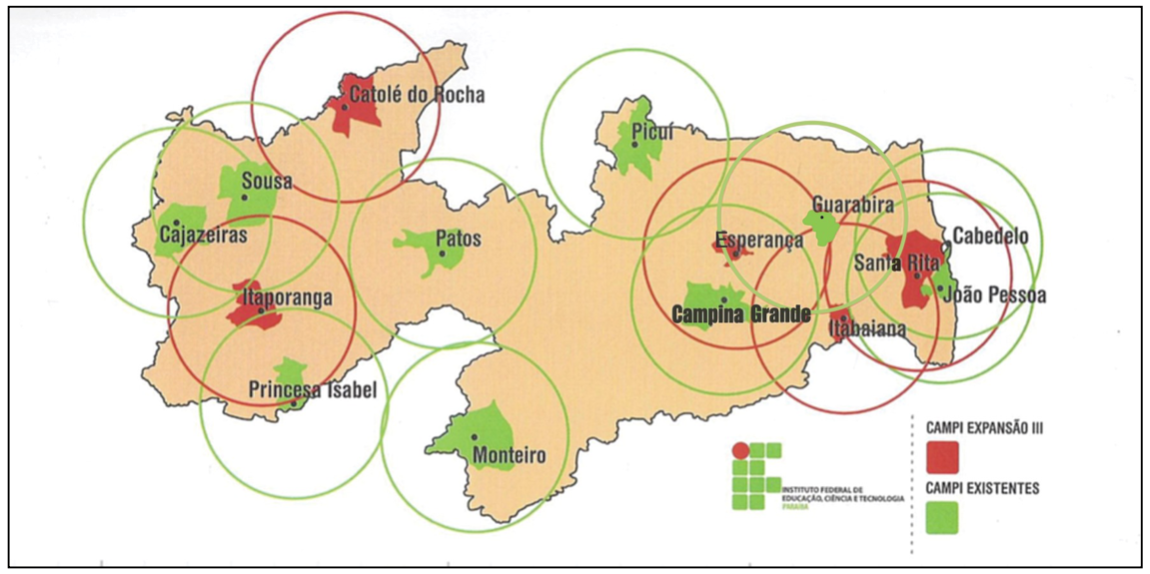
\includegraphics[height=2.5in]{imagens/campiIFPB1CG.png}
  \caption {Interiorização do IFPB. FONTE: IFPB (2014).}
  \label{fig:IFPB1}
\end{figure}

	As novas unidades educacionais levam a essas cidades e suas adjacências educação profissional nos níveis básico, técnico e tecnológico, proporcionando-lhes crescimento pessoal e formação profissional, oportunizando a essas regiões desenvolvimento econômico e social e, consequentemente, melhor qualidade de vida para a sua população.
	
	Nessa perspectiva, o IFPB atua nas áreas profissionais das Ciências Agrárias, Ciências Biológicas, Ciências da Saúde, Ciências Exatas e da Terra, Ciências Humanas, Ciências Sociais Aplicadas, Engenharias, Linguística, Letras e Artes. São ofertados cursos nos eixos tecnológicos de Recursos Naturais, Produção Cultural e Design, Gestão e Negócios, Infraestrutura, Produção Alimentícia, Controle e Processos Industriais, Produção Industrial, Hospitalidade e Lazer, Informação e Comunicação, Ambiente, Saúde e Segurança.

	Ao oferecer oportunidades em todos os níveis da aprendizagem, este Instituto permite o processo de verticalização do ensino. Assim, são ofertados Programas de Formação Continuada (FIC), PROEJA, Mulheres Mil, propiciando também o prosseguimento de estudos através do CERTIFIC, além de Cursos Técnicos, Cursos Superiores de Tecnologia, Licenciaturas, Bacharelados e estudos de Pós-Graduação Lato Sensu e Stricto Sensu.
	
	A Educação Profissional de Nível Técnico no IFPB é ofertada nas modalidades integrado e subsequente, nas áreas profissionais da construção civil, indústria, informática, meio ambiente, turismo e hospitalidade, saúde e cultura, considerando a carga horária mínima e as competências exigidas para cada área, de acordo com o Decreto n. 5.154/2004 e Resoluções CNE/CEB n. 04/1999 e n. 01/2005 do Conselho Nacional de Educação - CNE. 
	
	O IFPB oferece Cursos Técnicos em diversos segmentos da economia e áreas profissionais, em todos os seus Campi (A Tabela~\ref{tab:cursostec} na próxima página mostra os cursos técnicos ofertados pelos campi do IFPB).
	
\begin{table}[]
\centering
\caption{Cursos Técnicos Ofertados pelo IFPB.}
\label{tab:cursostec}
\begin{tabular}{|c|c|c|}
\hline
\rowcolor[HTML]{32CB00} 
\textbf{Campus}                                                          & \textbf{Eixos Tecnológicos}                                                & \textbf{Cursos}                                                                                                                                                                                    \\ \hline
                                                                         & Recursos Naturais                                                          & \begin{tabular}[c]{@{}c@{}}Técnico em Recursos Pesqueiros \\ (Integrado e Subsequente)\end{tabular}                                                                                                \\ \cline{2-3} 
\multirow{-2}{*}{Cabedelo}                                               & \begin{tabular}[c]{@{}c@{}}Ambiente, Saúde\\  e Segurança\end{tabular}     & \begin{tabular}[c]{@{}c@{}}Técnico em Meio Ambiente \\ (Integrado e Subsequente)\end{tabular}                                                                                                      \\ \hline
Cabedelo Centro                                                          & Infraestrutura                                                             & \begin{tabular}[c]{@{}c@{}}Técnico em Transporte Aquaviário \\ (Subsequente)\\ Técnico em Experimental em Náutica\\ (Subsequente)\end{tabular}                                                  \\ \hline
                                                                         & Infraestrutura                                                             & \begin{tabular}[c]{@{}c@{}}Técnico em Edificações \\ (Integrado e Subsequente)\end{tabular}                                                                                                        \\ \cline{2-3} 
                                                                         & \begin{tabular}[c]{@{}c@{}}Controle e Processos\\ Industriais\end{tabular} & \begin{tabular}[c]{@{}c@{}}Técnico em Eletromecânica \\ (Integrado e Subsequente)\end{tabular}                                                                                                     \\ \cline{2-3} 
\multirow{-3}{*}{Cajazeiras}                                             & \begin{tabular}[c]{@{}c@{}}Informação e\\ Comunicação\end{tabular}         & \begin{tabular}[c]{@{}c@{}}Técnico em Informática\\ (Integrado)\end{tabular}                                                                                                                       \\ \hline
                                                                         & Informação e Comunicação                                                   & \begin{tabular}[c]{@{}c@{}}Técnico em Manutenção \\ e Suporte de Informática \\ (Subsequente)\\ Técnico em Informática \\ (Integrado eSubsequente)\end{tabular}                                    \\ \cline{2-3} 
                                                                         & Recursos Naturais                                                          & \begin{tabular}[c]{@{}c@{}}Técnico em Mineração \\ (Integrado e Subsequente)\end{tabular}                                                                                                          \\ \cline{2-3} 
\multirow{-3}{*}{Campina Grande}                                         & Produção Industrial                                                        & \begin{tabular}[c]{@{}c@{}}Técnico em Petróleo e Gás \\ (Integrado)\end{tabular}                                                                                                                   \\ \hline
Catolé do Rocha                                                          & Infraestrutura                                                             & \begin{tabular}[c]{@{}c@{}}Técnico em Edificações \\ (Integrado)\end{tabular}                                                                                                                      \\ \hline
Esperança                                                                & Informação e Comunicação                                                   & \begin{tabular}[c]{@{}c@{}}Técnico em Informática \\ (Integrado e Subsequente)\end{tabular}                                                                                                        \\ \hline
                                                                         & Gestão e Negócios                                                          & \begin{tabular}[c]{@{}c@{}}Técnico em Contabilidade \\ (Integrado)\end{tabular}                                                                                                                    \\ \cline{2-3} 
                                                                         & Infraestrutura                                                             & \begin{tabular}[c]{@{}c@{}}Técnico em Edificações \\ (Integrado)\end{tabular}                                                                                                                      \\ \cline{2-3} 
\multirow{-3}{*}{Guarabira}                                              & \begin{tabular}[c]{@{}c@{}}Informação e\\ Comunicação\end{tabular}         & \begin{tabular}[c]{@{}c@{}}Técnico em Informática \\ (Integrado)\end{tabular}                                \\ \hline     
\end{tabular}
\end{table}


\begin{table}
\centering
\begin{tabular}{|c|c|c|}
\hline
\rowcolor[HTML]{32CB00} 
\textbf{Campus}                                                          & \textbf{Eixos Tecnológicos}                                                & \textbf{Cursos}  

                                                                                  \\ \hline
Itabaiana                                                                & Controle e Processos Industriais                                           & \begin{tabular}[c]{@{}c@{}}Técnico em Automação Industrial \\ (Integrado)\\ Técnico em Eletromecânica\\ (Integrado)\end{tabular}                                                                   \\ \hline
Itaporanga                                                               & Infraestrutura                                                             & \begin{tabular}[c]{@{}c@{}}Técnico em Edificações \\ (Integrado)\end{tabular}                                                                                                                      \\ \hline
                                                                         & Controle e Processos Industriais                                           & \begin{tabular}[c]{@{}c@{}}Técnico em Eletrotécnica\\ (Integrado e Subsequente)\\ Técnico em Mecânica\\ (Integrado e Subsequente)\\ Técnico em Eletrônica\\ (Integrado e Subsequente)\end{tabular} \\ \cline{2-3} 
                                                                         & Infraestrutura                                                             & \begin{tabular}[c]{@{}c@{}}Técnico em Edificações\\ (Integrado e Subsequente)\end{tabular}                                                                                                         \\ \cline{2-3} 
                                                                         & Gestão e Negócios                                                          & \begin{tabular}[c]{@{}c@{}}Técnico em Contabilidade \\ (Integrado)\\ Técnico em Secretariado \\ (Subsequente)\end{tabular}                                                                         \\ \cline{2-3} 
                                                                         & Produção Cultural e Design                                                 & \begin{tabular}[c]{@{}c@{}}Técnico em Instrumento Musical \\ (Integrado e Subsequente)\end{tabular}                                                                                                \\ \cline{2-3} 
                                                                         & Turismo, Hospitalidade e Lazer                                             & \begin{tabular}[c]{@{}c@{}}Técnico em Eventos\\ (PROEJA)\end{tabular}                                                                                                                              \\ \cline{2-3} 
\multirow{-6}{*}{João Pessoa}                                            & Ambiente, Saúde e Segurança                                                & \begin{tabular}[c]{@{}c@{}}Técnico em Equipamentos Biomédicos\\ (Subsequente)\\ Técnico em Controle Ambiental \\ (Integrado)\end{tabular}                                                          \\ \hline
\begin{tabular}[c]{@{}c@{}}Campus Avançado\\  de Mangabeira\end{tabular} & Ambiente e Saúde                                                           & \begin{tabular}[c]{@{}c@{}}Técnico em Cuidados de Idosos \\ (Subsequente)\end{tabular}                                                                                                            \\ \hline
                                                                         & Informação e Comunicação                                                   & \begin{tabular}[c]{@{}c@{}}Técnico em Manutenção \\ e Suporte em Informática \\ (Integrado e Subsequente)\end{tabular}                                                                             \\ \cline{2-3} 
\multirow{-2}{*}{Monteiro}                                               & Produção Cultural e Design                                                 & \begin{tabular}[c]{@{}c@{}}Técnico em Instrumento Musical\\ (Integrado)\end{tabular}                                                                                                      \\ \hline
         


\end{tabular}
\end{table}


\begin{table}
\centering
\begin{tabular}{|c|c|c|}
\hline
\rowcolor[HTML]{32CB00} 
\textbf{Campus}                                                          & \textbf{Eixos Tecnológicos}                                                & \textbf{Cursos}  




                                                                     \\ \hline
                                                                         & Controle e Processos Industriais                                           & \begin{tabular}[c]{@{}c@{}}Técnico em Eletrotécnica \\ (Integrado e Subsequente)\end{tabular}                                                                                                      \\ \cline{2-3} 
                                                                         & Informação e Comunicação                                                   & \begin{tabular}[c]{@{}c@{}}Técnico em Manutenção \\ e Suporte em Informática \\ (Integrado e Subsequente)\end{tabular}                                                                             \\ \cline{2-3} 
                                                                         & Infraestrutura                                                             & \begin{tabular}[c]{@{}c@{}}Técnico em Edificações\\ (Integrado e Subsequente)\end{tabular}                                                                                                         \\ \cline{2-3} 
\multirow{-4}{*}{Patos}                                                  & Segurança                                                                  & \begin{tabular}[c]{@{}c@{}}Técnico em Segurança do Trabalho \\ (Integrado)\end{tabular}                                                                                                            \\ \hline
                                                                         & Informação e Comunicação                                                   & \begin{tabular}[c]{@{}c@{}}Técnico em Informática\\ (Integrado)\\ Técnico em Manutenção \\ e Suporte em Informática \\ (Subsequente)\end{tabular}                                                  \\ \cline{2-3} 
                                                                         & Infraestrutura                                                             & \begin{tabular}[c]{@{}c@{}}Técnico em Edificações\\ (Integrado)\\ Técnico em Geologia\\ (Integrado)\end{tabular}                                                                                   \\ \cline{2-3} 
\multirow{-3}{*}{Picuí}                                                  & Recursos Naturais                                                          & \begin{tabular}[c]{@{}c@{}}Técnico em Mineração\\ (Subsequente)\end{tabular}                                                                                                                       \\ \hline
                                                                         & Informação e Comunicação                                                   & \begin{tabular}[c]{@{}c@{}}Técnico em Manutenção \\ e Suporte em Informática\\ (Subsequente)\end{tabular}                                                                                          \\ \cline{2-3} 
                                                                         & Ambiente, Saúde e Segurança                                                & \begin{tabular}[c]{@{}c@{}}Técnico em Controle Ambiental\\ (Integrado)\end{tabular}                                                                                                                \\ \cline{2-3} 
\multirow{-3}{*}{Princesa Isabel}                                        & Infraestrutura                                                             & \begin{tabular}[c]{@{}c@{}}Técnico em Edificações\\ (Integrado e Subsequente)\end{tabular}                                                                                                         \\ \hline
                                                                         & Informação e Comunicação                                                   & \begin{tabular}[c]{@{}c@{}}Técnico em Informática\\ (Integrado)\end{tabular}                                                                                                                       \\ \cline{2-3} 
\multirow{-2}{*}{Santa Rita}                                             & Ambiente, Saúde e Segurança                                                & \begin{tabular}[c]{@{}c@{}}Técnico em Meio Ambiente\\ (Integrado)\end{tabular}                                                                                                                     \\ \hline
                                                                         & Informação e Comunicação                                                   & \begin{tabular}[c]{@{}c@{}}Técnico em Informática\\ (Integrado e Subsequente)\end{tabular}                                                                                                         \\ \cline{2-3} 
                                                                         & Recursos Naturais                                                          & \begin{tabular}[c]{@{}c@{}}Técnico em Agropecuária\\ (Integrado e Subsequente)\end{tabular}                                                                                                        \\ \cline{2-3} 
                                                                         & Ambiente, Saúde e Segurança                                                & \begin{tabular}[c]{@{}c@{}}Técnico em Meio Ambiente\\ (Integrado)\\ Técnico em Agroindústria\\ (PROEJA)\end{tabular}                                                                               \\ \cline{2-3} 
\multirow{-4}{*}{Sousa}                                                  & Produção Alimentícia                                                       & \begin{tabular}[c]{@{}c@{}}Técnico em Agroindústria\\ (Integrado)\end{tabular}                                                                                                                     \\ \hline
\end{tabular}
\end{table}


	A Educação Profissional Técnica Integrada ao Ensino Médio é oferecida para estudantes que tenham concluído o Ensino Fundamental. A organização dos cursos conduz o aluno a uma habilitação profissional técnica de nível médio, e lhe dará o direito à continuidade de estudos na educação superior. 
	
	%A Educação Profissional de Nível Técnico no IFPB corresponde à oferta de cursos técnicos, considerando a carga horária mínima e o perfil profissional exigidos para cada eixo tecnológico, de acordo com o Catálogo Nacional dos Cursos Técnicos – Resolução do CNE/CEB Nº 4, DE 6 DE JUNHO DE 2012.
	
%	O currículo dos Cursos Técnicos Integrados ao Ensino Médio está estruturado em regime anual com duração de 03 (três) anos, integrando a formação geral com uma carga horária mínima de 2.400 horas e a formação técnica, conforme a carga horária mínima exigida no Catálogo Nacional dos Cursos Técnicos – CNCT – para a respectiva habilitação profissional, acrescida da carga horária destinada ao estágio curricular e/ou Trabalho de Conclusão de Curso – TCC. 
	
	%Além disso, esse currículo está definido por disciplinas orientadas pelos perfis de conclusão e distribuídas na matriz curricular com as respectivas cargas horárias, propiciando a visualização geral do curso.
	
	A Educação Profissional ofertada para a Educação de Jovens e Adultos, respeitando suas especificidades definidas no Decreto nº 5.840, de 13 de julho de 2006, é ofertada com as mesmas características do Ensino Técnico Integrado estabelecidas no Decreto Nº 5.154, de 23 de julho de 2004. Nesse sentido, o atendimento a essa clientela pressupõe ações voltadas para o seu projeto de vida e para as necessidades urgentes de (re)inserção e de (re)qualificação, visando à complementação da renda familiar ou ao provimento de seu sustento. Dessa forma, o ensino aponta para um projeto capaz de vislumbrar o trabalho como princípio educativo. Assim, estaremos, enquanto instituição de ensino, resgatando a nossa função social e promovendo dignidade e cidadania. Atualmente, o IFPB oferta esta modalidade de ensino contemplando os cursos: Técnico Integrado em Eventos, em João Pessoa; Operação de Microcomputadores, em Campina Grande; Desenho de Construção Civil, em Cajazeiras, e Agroindústria, em Sousa. 
	
	\newpage
	
	Em se tratando de educação superior, o IFPB dispõe de Cursos de Tecnologia, Licenciatura, Bacharelado e Engenharia (a Tabela~\ref{tab:cursossuperiores} mostra os cursos superiores oferecidos pelos campi do IFPB). Com esta Educação Profissional Tecnológica de Graduação, os Cursos Superiores de Tecnologia integram as diferentes formas de educação ao trabalho, à ciência e à tecnologia e visam, segundo suas diretrizes curriculares, garantir aos cidadãos o direito à aquisição de competências profissionais que os tornem aptos para a inserção no mercado de trabalho. Com a Educação Profissional Tecnológica de Graduação, a Instituição tem galgado seu espaço, construindo uma educação gratuita e de qualidade, assentada nos mais modernos fundamentos científicos e tecnológicos, potencializando-se em opção de qualidade para as diversas gerações.

	A oferta dos Cursos de Licenciatura visa atender à Lei 11.892/2008 e foi criada com o objetivo de minimizar a falta de profissionais de educação para o exercício da docência nas Escolas de Educação Básica. As Licenciaturas, cujo objetivo é a habilitação de profissionais de diversas áreas do conhecimento para atuar no magistério, são ofertadas àqueles que possuem diploma de Ensino Médio. Dessa forma os programas de formação pedagógica foram regulamentados pela Resolução nº 2, de 07 de julho de 1999, alterando a Portaria 432, de 19 de julho de 1971, que regulamentava a formação de docentes para as disciplinas do currículo da educação profissional. Vale salientar que, mesmo antes da edição da referida Lei, atuando com uma visão de futuro, o IFPB já ofertava o Curso de Licenciatura em Química.
	
	Além dos Cursos Superiores de Tecnologia e Licenciaturas, atualmente o IFPB oferece o Bacharelado em Administração e em Engenharia Elétrica no campus João Pessoa, o bacharelado em Medicina Veterinária no campus Sousa, o bacharelado em Engenharia Civil no campus Cajazeiras e o bacharelado em Engenharia de Computação no campus Campina Grande. 
	
	A duração, carga horária e tempo de integralização deste cursos presenciais, no âmbito do IFPB, atendem ao Parecer CNE/CES nº 08/2007 e Resolução CNE/CES Nº 02/2007. Os estágios e atividades complementares dos referidos cursos, na modalidade presencial, não deverão exceder a 20\% (vinte por cento) da carga horária total do curso, salvo nos casos de determinações legais em contrário, tomando por base a Resolução CNE/CES Nº 02/2007. Em relação aos Cursos de Engenharia, o IFPB adota como referencial o Parecer CNE/CES nº 1.362/2001 que estabelece Diretrizes Curriculares Nacionais dos Cursos de Engenharia.

\begin{table}[]
\centering
\caption{Cursos Superiores ofertados pelo IFPB}
\label{tab:cursossuperiores}
\begin{tabular}{|c|c|c|}
\hline
\rowcolor[HTML]{32CB00} 
\textbf{Campus}                  & \textbf{Eixos Tecnológicos}                                                 & \textbf{Cursos}                                                                                                                                                      \\ \hline
                                 & Produção Cultural                                                  & \begin{tabular}[c]{@{}c@{}}CST em Design Gráfico\end{tabular}                                                                              \\ \cline{2-3} 
\multirow{-2}{*}{Cabedelo}       & Licenciatura                                                           & Licenciatura em Ciências Biológicas          
                                                                                                                                            \\ \hline
                                 & \begin{tabular}[c]{@{}c@{}}Informação e\\  Comunicação\end{tabular}         & \begin{tabular}[c]{@{}c@{}}CST em Análise e \\ Desenvolvimento de Sistemas\end{tabular}                                                                              \\ \cline{2-3} 
                                 & \begin{tabular}[c]{@{}c@{}}Controle e Processos \\ Industriais\end{tabular} & CST em Automação Industrial                                                                                                                                          \\ \cline{2-3} 
                                 & Licenciatura                                                                & Licenciatura em Matemática                                                                                                                                           \\ \cline{2-3} 
\multirow{-4}{*}{Cajazeiras}     & Bacharelado                                                                 & Bacharelado em Engenharia Civil                                                                                                                                      \\ \hline
                                 & Informação e Comunicação                                                    & CST em Telemática                                                                                                                                                    \\ \cline{2-3} 
                                 & Licenciatura                                                                & \begin{tabular}[c]{@{}c@{}}Licenciatura em Física\\ Licenciatura em Matemática\end{tabular}                                                                          \\ \cline{2-3} 
                                 & Infraestrutura                                                              & CST em Construção de Edifícios                                                                                                                                       \\ \cline{2-3} 
\multirow{-4}{*}{Campina Grande} & Bacharelado                                                                 & \begin{tabular}[c]{@{}c@{}}Bacharelado em \\ Engenharia de Computação\end{tabular}                                                                                   \\ \hline
Guarabira                        & Gestão e Negócios                                                           & CST em Gestão Comercial                                                                                                                                              \\ \hline
                                 & Controle e Processos Industriais                                            & CST em Automação Industrial                                                                                                                                          \\ \cline{2-3} 
                                 & Licenciatura                                                                & Licenciatura em Química                                                                                                                                              \\ \cline{2-3} 
                                 & Infraestrutura                                                              & CST em Construção de Edifícios                                                                                                                                       \\ \cline{2-3} 
                                 & Gestão e Negócios                                                           & CST em Negócios Imobiliários                                                                                                                                         \\ \cline{2-3} 
                                 & Produção Cultural e Design                                                  & CST em Design de Interiores                                                                                                                                          \\ \cline{2-3} 
                                 & Bacharelado                                                                 & \begin{tabular}[c]{@{}c@{}}Bacharelado em Administração\\ Bacharelado em Engenharia Elétrica\end{tabular}                                                            \\ \cline{2-3} 
                                 & Informação e Comunicação                                                    & \begin{tabular}[c]{@{}c@{}}CST em Geoprocessamento\\ CST em Redes de Computadores\\ CST em Sistemas de Telecomunicações\\ CST em Sistemas para Internet\end{tabular} \\ \cline{2-3} 
\multirow{-8}{*}{João Pessoa}    & Ambiente e Saúde                                                            & CST em Gestão Ambiental                                                                                                                                              \\ \hline
                                 & Informação e Comunicação                                                    & \begin{tabular}[c]{@{}c@{}}CST em Análise e \\ Desenvolvimento de Sistemas\end{tabular}                                                                              \\ \cline{2-3} 
\multirow{-2}{*}{Monteiro}       & Infraestrutura                                                              & CST em Construção de Edifícios                                                                                                                                       \\ \hline
Patos                            & Segurança                                                                   & CST em Segurança do Trabalho                                                                                                                                         \\ \hline
Picuí                            & Recursos Naturais                                                           & CST em Agroecologia                                                                                                                                                  \\ \hline
Princesa Isabel                  & Ambiente e Saúde                                                            & CST em Gestão Ambiental                                                                                                                                              \\ \hline
                                 & Recursos Naturais                                                           & CST em Agroecologia                                                                                                                                                  \\ \cline{2-3} 
                                 & Licenciatura                                                                & \begin{tabular}[c]{@{}c@{}}Licenciatura em Química\\ Licenciatura em Educação Física\end{tabular}                                                                    \\ \cline{2-3} 
                                 & Produção Alimentícia                                                        & CST em Alimentos                                                                                                                                                     \\ \cline{2-3} 
\multirow{-4}{*}{Sousa}          & Bacharelado                                                                 & Bacharelado em Medicina Veterinária                                                                                                                                  \\ \hline
\end{tabular}
\end{table}


	Após a consolidação do ensino superior em nível de graduação, o IFPB iniciou a oferta de cursos de pós-graduação, nas suas diversas áreas, com a finalidade de atender à demanda social por especialistas. Os cursos de especialização lato sensu em Segurança da Informação, Educação Profissional e Gestão Pública iniciaram uma série de cursos de pós-graduação ofertados por esse Instituto. O IFPB também oferta atualmente o curso de Mestrado em Engenharia Elétrica, na modalidade stricto sensu.
	
	Para uma instituição de ensino profissionalizante que prima pela qualidade e busca a todo tempo incrementá-la, é estratégico para o seu dinamismo ter um programa de incentivo e difusão da cultura, da pesquisa científica e tecnológica. Nesse sentido, o IFPB tem buscado construir e difundir conhecimentos, apoiar tecnologicamente o setor produtivo, propiciar a iniciação científica aos discentes, fazer a realimentação curricular dos cursos, obter recursos para a Instituição e incentivar a formação em pós-graduação dos servidores.
	
	Assim, a Pró-reitoria de Pesquisa, Inovação e Pós-graduação, setor tático responsável pelas ações para o desenvolvimento da pesquisa científica e tecnológica e pela pós-graduação no IFPB, apresenta uma proposta cujo instrumento norteador são as ações realizadas nos próprios campi, de modo que os grupos ou núcleos de pesquisa constituem-se células mater nesse processo de desenvolvimento. Portanto, buscar formas de incentivar a sua criação/consolidação e apoiar o seu desenvolvimento torna-se crucial para o sucesso de qualquer plano institucional de pesquisa científica e tecnológica, inovação e pós-graduação.
	
	Naturalmente, associa-se pesquisa aos cursos superiores ou aos programas de pós-graduação, contudo, ressalta-se que a pesquisa científica e tecnológica já vem sendo realizada em todas as modalidades de ensino do IFPB: Ensino Médio, Ensino Técnico, Ensino de Graduação (Tecnológico, Bacharelado e Licenciatura) e Ensino de Pós-Graduação (Stricto Sensu e Lato Sensu).
	
	Assim, o IFPB há muito tem demonstrado o seu potencial no campo da pesquisa científica e tecnológica. Possui uma infraestrutura física de laboratórios de razoável a boa e um quadro efetivo de recursos humanos bem qualificado. Atualmente, o IFPB possui 113 (cento e treze) grupos de pesquisa cadastrados no CNPq e certificados pela Instituição, nas seguintes áreas: 
	
	\begin{itemize}
		\item Administração - 3
		\item Agronomia	- 3
		\item Arquitetura e Urbanismo - 1
		\item Astronomia - 2
		\item Botânica - 1
		\item Ciência da Computação - 19
		\item Ciência da Informação - 1
		\item Ciência e Tecnologia de Alimentos - 2
		\item Desenho Industrial - 1
		\item Ecologia - 1
		\item Educação - 12
		\item Educação Física - 1
		\item Engenharia Biomédica - 1
		\item Engenharia Civil - 2
		\item Engenharia de Materiais e Metalúrgica - 1
		\item Engenharia de Minas - 2
		\item Engenharia Elétrica - 16
		\item Engenharia Mecânica - 7
		\item Engenharia Sanitária - 2
		\item Filosofia - 3
		\item Geociências - 10
		\item História - 1
		\item Letras - 3
		\item Lingüística - 3
		\item Medicina Veterinária - 2
		\item Planejamento Urbano e Regional - 1
		\item Química - 6
		\item Recursos Pesqueiros e Engenharia de Pesca - 3
		\item Saúde Coletiva - 1
		\item Serviço Social - 1
		\item Sociologia - 1
	\end{itemize}

	Esses grupos têm apresentado produção acadêmica constante e consistente, inclusive proporcionando aos discentes a iniciação científica e servindo de incentivo para a formação de novos grupos.
	
	A Instituição conta, ainda, com um veículo impresso para divulgação de trabalhos científicos e tecnológicos, que é a Revista Principia.
	
	É sobre esta base de ciência e tecnologia, construída nos últimos anos, que o IFPB trabalha para reforçar a sua capacidade de produção de pesquisas científicas e tecnológicas e de inovação tecnológica, voltadas ao desenvolvimento educacional, econômico e social da nossa região de abrangência.

	Além das atividades pertinentes à Pesquisa, o IFPB tem atuado, também, junto à Extensão, desenvolvendo, de acordo com as dimensões da extensão estabelecidas pelo FORPROEXT (Fórum de Dirigentes de Extensão da Rede de Educação Profissional e Tecnológica), os seguintes projetos:
	
	\begin{itemize}
		\item Projetos Tecnológicos: desenvolvimento de atividades de investigação científica, técnica e tecnológica, em parceria com instituições públicas ou privadas que tenham interface de aplicação.
		\item Serviços Tecnológicos: oferta de serviços de consultoria, assessoria, e outros serviços de cunho técnico e tecnológico, para o mundo produtivo.
		\item Eventos: realização de ações de interesse técnico, social, científico, esportivo, artístico e cultural, favorecendo a participação da comunidade externa e/ou interna.
		\item Projetos Sociais: projetos que agregam um conjunto de ações, técnicas e metodologias transformadoras, desenvolvidas e/ou aplicadas na interação com a população e apropriadas por ela, que representam soluções para inclusão social, geração de oportunidades e melhoria das condições de vida.
		\item Cursos de Extensão: ação pedagógica de caráter teórico e prático de oferta não regular, que objetiva a capacitação de cidadãos.
		\item Projetos Culturais Artísticos e Esportivos: compreende ações de apoio e promoção de eventos de caráter cultural, cívico, artístico e desportivo.
		\item Visitas Técnicas e Gerenciais: interação das áreas educacionais da Instituição com o mundo do trabalho.
		\item Empreendedorismo: compreende o apoio técnico educacional com vistas à formação empreendedora, bem como ao desenvolvimento de serviços e produtos tecnológicos.
		\item Acompanhamento de egressos: constitui-se no conjunto de ações implementadas que visam acompanhar o desenvolvimento profissional do egresso, na perspectiva de identificar cenários junto ao mundo do trabalho e retroalimentar o processo de ensino, pesquisa e extensão.
	\end{itemize}

\paragraph{Síntese Histórica do IFPB - Campus Guarabira}\

Guarabira foi a primeira cidade integrante do Plano de Expansão III a iniciar suas atividades educativas, portanto torna-se necessário discorrer sobre os aspectos e peculiaridades que a caracterizam.

O IFPB Campus Guarabira foi inaugurado em 10 de outubro de 2011 (na época como Núcleo Avançado) e atualmente funciona na Rua José Américo de Almeida, S/N, no Bairro do Nordeste I, no Centro de Vocação Tecnológica - CVT (antigo CAIC).

Os cursos ofertados pelo IFPB - Campus Guarabira devem atender às carências da região, levando em consideração o contexto socioeconômico bem como sua viabilidade nessa fase inicial.

	Guarabira é um município que está localizado no Piemonte da Borborema, na microrregião que recebe o seu nome Microrregião de Guarabira. Seu nome, de origem tupi, quer dizer berço das garças, ``guará-pora'' ou ``bira'', isto é, moradia dos guarás. Com uma área de 149,50 $km^2$, o município ocupa o 115~{\degree} lugar em extensão territorial no Estado e possui uma posição geográfica invejável, pois fica a apenas 96 km de distância de João Pessoa (Capital Paraibana), 100 km de Campina Grande (maior cidade do interior nordestino), 199 km do Recife (Capital de Pernambuco), 145 km de Natal (um dos maiores polos turísticos do Brasil) e a 230 km de Caruaru (grande centro comercial nordestino). A sede do município fica a 97 metros de altitude, 06~{\degree} 51’17" Sul e 35~{\degree} 29’24" Oeste.

	É chamada Rainha do Brejo pelo fato de ser a principal cidade-polo de uma região que se caracteriza pela regularidade de chuvas. Guarabira é polo de educação na Região do Brejo, atendendo alunos do ensino fundamental até pós-graduação em ensino superior, situação que atrai estudantes de todo o estado da Paraíba, bem como de outros estados da federação. A cidade possui universidades privadas e públicas, incluindo o Campus III da Universidade Estadual da Paraíba - UEPB, contando com os cursos de Direito, História, Geografia, Letras e Pedagogia.

	A chegada do IFPB a Guarabira traz inovação e tecnologia, formando profissionais capacitados para atuarem diretamente no contexto econômico da região, ou seja, nos diversos setores: comércio, indústria e serviços; geograficamente, está localizada em uma região em que polariza mais de 30 cidades, todas tendo um forte vínculo com o município.

	Atualmente o Campus Guarabira oferta três cursos técnicos integrados ao ensino médio: Informática, Edificações e Contabilidade e o Curso Superior de Tecnologia em Gestão Comercial. Com o progresso e o dinamismo presente nas capitais e principais cidades dos estados nordestinos, é primordial para a consolidação desta realidade, o desenvolvimento da educação por meio da formação de novos profissionais para atender a realidade local. Neste contexto, o Curso Superior de Tecnologia em Sistemas para Internet vem suprir demandas reais nesse cenário.

\subsubsection{Cenário sócio-econômico da região}

	A Paraíba está situada no Nordeste brasileiro, limitada pelos Estados de Pernambuco, Rio Grande do Norte e Ceará, além de ter sua costa banhada pelo Oceano Atlântico. Em 2010, contava com uma população estimada em 3.914.421 (três milhões, novecentos e quatorze mil e quatrocentos e vinte e um) habitantes, segundo o Censo de 2010, divulgado pelo IBGE.

	Apesar de possuir uma economia pequena, se comparada com aquelas dos estados mais desenvolvidos do país, a Paraíba tem experimentado índices de crescimento bastante expressivos. A variação do Produto Interno Bruto deste Estado, em comparação aos índices apresentados para o Nordeste e o Brasil, pode ser vista com o auxílio do Quadro 3 (Contas Regionais do Brasil 2010-2013 - IBGE, 2013).

\begin{table}[h]
\caption{Produto Interno Bruto per capita do Brasil, Nordeste e Paraíba.}
\begin{tabular}{|
>{\columncolor[HTML]{FFFFFF}}l |
>{\columncolor[HTML]{FFFFFF}}l |
>{\columncolor[HTML]{FFFFFF}}l |
>{\columncolor[HTML]{FFFFFF}}l |
>{\columncolor[HTML]{FFFFFF}}l |}
\hline
\textbf{\begin{tabular}[c]{@{}l@{}}Ano Moeda\\ PIB per capita\end{tabular}} & \textbf{2010} & \textbf{2011} & \textbf{2012} & \textbf{2013}  \\ \hline
Brasil                                                                      & 20.371,64     & 22.734,56     & 24.779,53     & 26.445,72     \\ \hline
Nordeste                                                                    & 9.848,97      & 10.904,56      & 12.099,67      & 12.954,80     \\ \hline
Paraíba                                                                     & 8.899,93      & 9.790,27      & 11.132,89      & 11.834,54      \\ \hline
\end{tabular}
\end{table}

No tocante aos aspectos econômico, social e político, a Paraíba está dividida em 4 (quatro) mesorregiões, assim denominadas, de acordo com a classificação estabelecida pelo IBGE: Mata Paraibana, Agreste Paraibano, Borborema e Sertão Paraibano. Essas mesorregiões estão, por sua vez, desagregadas em 23 microrregiões geográficas. Diante da prevalência dos problemas enfrentados pela população que habita as áreas semi-áridas do estado e da necessidade de solucionar a crise econômica que afeta a Zona da Mata e a Região do Brejo, optou-se por adotar a divisão clássica do estado da Paraíba e agregar seus principais espaços econômicos nas seguintes zonas geoeconômicas: Litoral-Mata, Agreste-Brejo e Semi-Árida. A divisão das mesorregiões pode ser visto na Figura~\ref{fig:meso}.

\begin{figure}
  \centering
  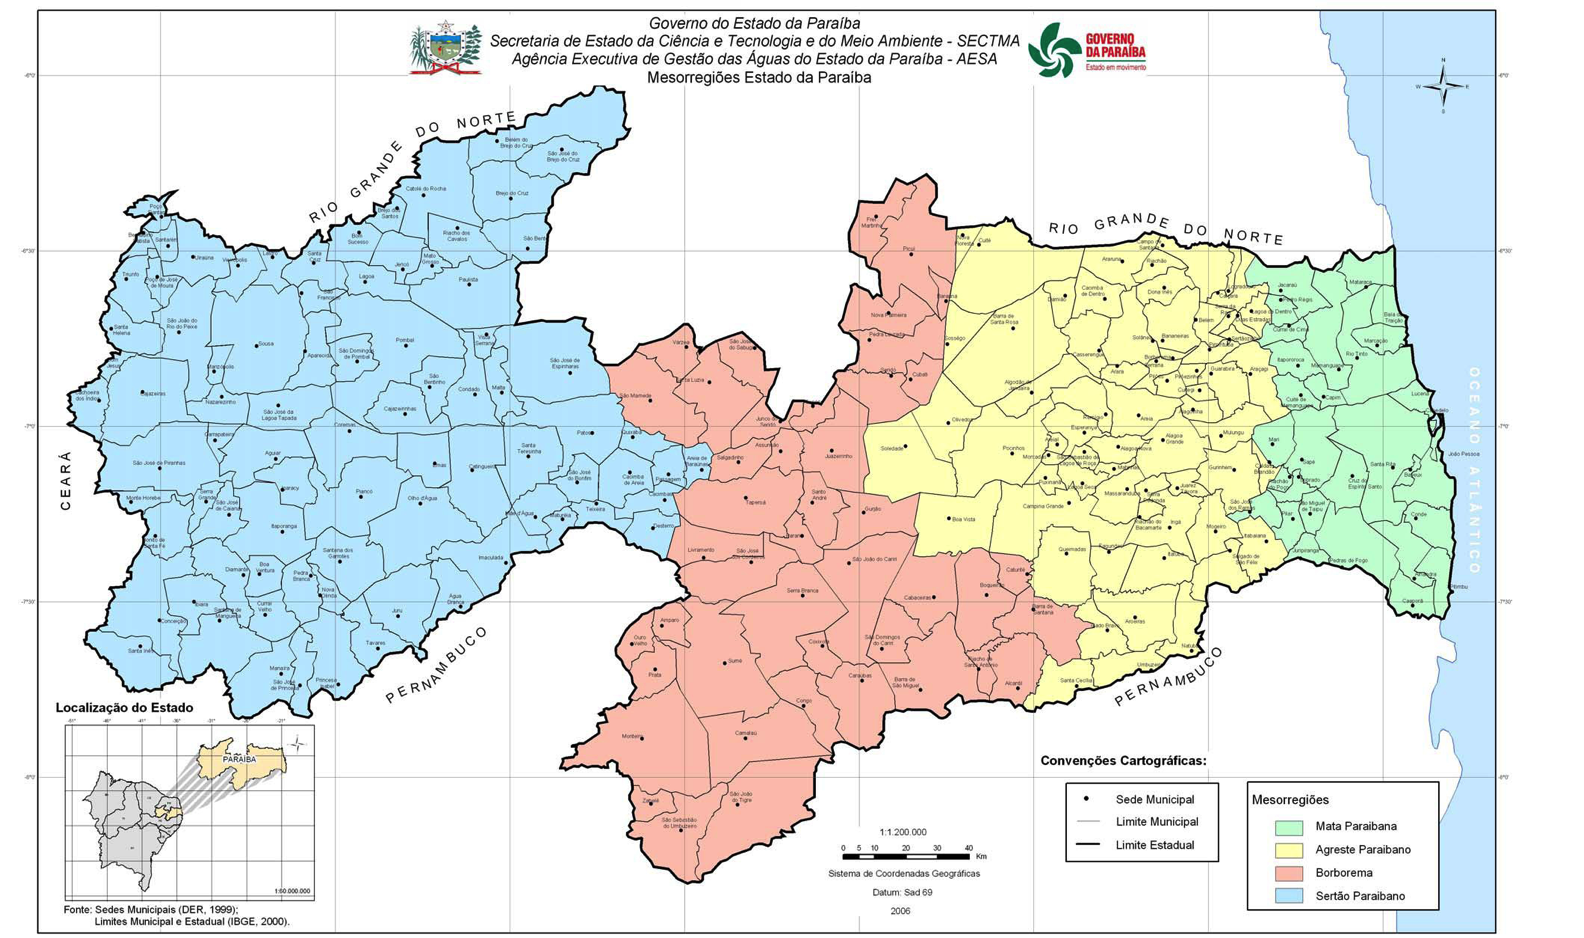
\includegraphics[height=3.0in]{imagens/mesorregioes.png}
  \caption { Mesorregiões econômicas da Paraíba. FONTE: PDI-IFPB (2010)}
  \label{fig:meso}
\end{figure}

A Zona Litoral-Mata corresponde à Mesorregião Mata Paraibana, definida pelo IBGE e integrada pelas seguintes Microrregiões Geográficas: Litoral Norte, Sapé, João Pessoa e Litoral Sul, que englobam 30 dos 223 municípios do Estado, ou seja, 13,45~\% do total. Com uma superfície de 5.242 $km^2$ (9,3~\% do território do Estado), em 2000 abrigava uma população de 1.196.594 habitantes, o que significa uma densidade de 228,3 $hab/km^2$. O grande aglomerado urbano da Capital do Estado é um dos principais responsáveis por essa concentração populacional.

A Zona do Agreste-Brejo abrange quase que integralmente as Microrregiões constitutivas da Mesorregião do Agreste, tal como definida pelo IBGE: Esperança, Brejo Paraibano, Guarabira, Campina Grande, Itabaiana e Umbuzeiro. Essas seis microrregiões reúnem 48 municípios (21,5~\% do total). Para os efeitos da classificação aqui adotada, a Zona do Agreste-Brejo deixa de englobar as Microrregiões do Curimataú Ocidental e do Curimataú Oriental, que passam a integrar a Zona Semi-Árida. Com isto, a Zona do Agreste-Brejo passa a ter uma área de 7.684 $km^2$ (13,6~\% da superfície total do estado) e no ano de 2000 uma população de 950.494 habitantes (IDEME, 2001), consistindo em uma zona de grande concentração populacional, pois possuía, no referido ano, uma densidade demográfica de 123,7 $hab/km^2$, correspondendo a 54~\% da observada na Zona Litoral-Mata. A densidade demográfica do Agreste-Brejo é 2 vezes superior à média do Estado. O peso populacional do Agreste-Brejo é, em grande parte, devido à cidade de Campina Grande, onde vivem 37,4~\% dos habitantes dessa zona.

A Zona Semi-Árida é a mais extensa em área, com 43.513,65 $km^2$ (77,1~\% do total do Estado), assim como a dotada de maior número absoluto de habitantes. Sua população, em 2000, era de 1.296.737 pessoas (37,6~\% do total), o que representava uma densidade demográfica de 29,8 $hab/km^2$. Esse indicador espelha as dificuldades enfrentadas pela população que vive naquela zona, pois dada à escassez relativa de recursos naturais que a caracteriza, ela apresenta a menor densidade demográfica entre as zonas geo-econômicas consideradas. Sua população está sujeita a condições de insustentabilidade, tanto econômica quanto social, bem mais difíceis de controlar do que as encontradas nas Zonas Litoral-Mata e Agreste-Brejo. Comparado aos demais espaços semi-áridos do Nordeste, o da Paraíba é um dos mais afetados pela degradação ambiental. Da categoria semiárida paraibana aqui considerada, fazem parte os seguintes espaços: Mesorregião do Sertão Paraibano (Microrregiões Geográficas de Catolé do Rocha, Cajazeiras, Sousa, Patos, Piancó, Itaporanga e Serra do Teixeira); Mesorregião da Borborema (Microrregiões do Seridó Ocidental, Seridó Oriental, Cariri Ocidental e Cariri Oriental); e as terras do Planalto da Borborema, conhecidas como Curimataú, representadas pelas Microrregiões do Curimataú Ocidental e do Curimataú Oriental, que integram a Mesorregião do Agreste, tal como classificada pelo IBGE.

Para efeito de análise de mercado, podemos dividir a Paraíba em três mesorregiões distintas: a zona da mata, região polarizada pela capital João Pessoa; o agreste, região central do estado, polarizada pela cidade de Campina Grande e o sertão, com suas características próprias, polarizada pela cidade de Patos.

O sertão se caracteriza pelo baixo índice de industrialização, em relação a sua extensão e densidade populacional. Basicamente, observam-se a presença de indústrias de beneficiamento mineral (área na qual o Estado apresenta um considerável potencial de exploração), além da indústria de alimentos e bebidas, ambas com baixos índices de automação. A mesorregião conta com três distritos industriais: Patos, com aproximadamente 35~ha; Sousa com 32,5~ha e Cajazeiras com 21,39~ha.

Embora dotadas de razoável infraestrutura, as indústrias dessa mesorregião não declararam investimentos em melhorias ou ampliações da capacidade produtiva no protocolo de intenções industriais entre 1996 e 1998, e apenas uma delas recebeu incentivos do FAIM (Fundo de Apoio ao Desenvolvimento Industrial da Paraíba) no mesmo período, o que resultou em menos de 100 novas vagas de emprego na cidade de Cajazeiras.

Na área educacional, o sertão paraibano é atendido pela Rede Estadual de Escolas Públicas, responsável pelo Ensino Médio, na maioria das cidades da região. A Rede Municipal é responsável pelo Ensino Básico e Fundamental, ofertado na zona urbana e rural da maioria dos municípios. A região conta ainda com dois campi do IFPB, em Sousa e Cajazeiras, que servem a boa parte da região do sertão, além de unidades do SENAI, SENAC, SEBRAE e rede privada, sendo também atendida por projetos do SENAR e do SENAT. No Ensino Superior, além do Campus de Cajazeiras, que oferta dois Cursos Superiores de Tecnologia (Análise e Desenvolvimento de Sistemas e Automação Industrial), um Curso Superior de Bacharelado em Engenharia Civil e um Curso Superior de Licenciatura em Matemática, o sertão conta com vários campi da Universidade Federal de Campina Grande (UFCG), localizados nas cidades de Patos, Sousa e Cajazeiras, onde são oferecidos cursos como Engenharia Florestal, Veterinária, Direito, Pedagogia, entre outros. A cidade de Patos conta ainda com a Fundação Francisco Mascarenhas, que oferece cursos de graduação e pós-graduação.

A mesorregião do agreste paraibano apresenta um grau de urbanização e desenvolvimento maior que a do sertão e comparável à zona da mata. Com três distritos industriais – todos situados na cidade de Campina Grande –, ela apresenta indústrias de transformação nas áreas de química, eletro-eletrônicos, mineração, têxtil, metal-mecânica, produtos alimentícios, bebidas, materiais plásticos, papel e papelão, cerâmica, couro calçado, editorial e gráfico e borracha. O índice de automação das indústrias varia de baixo a médio, com algumas indústrias empregando tecnologias de ponta no seu processo produtivo.

Desta forma, Campina Grande, polo da região, possui uma grande demanda de serviços técnicos na área de eletrônica e informática, seja para atender ao parque industrial, seja na prestação de serviços de manutenção ou desenvolvimento de equipamentos e sistemas. Observando o número de empresas assistidas pelos recursos do FAIM entre os anos de 1996 e 1998, cerca de 34 indústrias de diversos setores da economia foram beneficiadas, gerando cerca de 6.500 empregos somente nesta mesorregião.

%Além do mais, o agreste, capitaneado por Campina Grande, conta com a presença de unidades do SENAI, SENAC, SEBRAE, além de outras instituições de educação profissional, públicas e privadas, tendo se destacado por sua vocação educacional, ampliando sua área de atendimento aos demais estados da região Nordeste e do país.

Situação similar à do agreste ocorre na mesorregião da zona da mata. Os seis distritos industriais existentes nas cidades de João Pessoa, Conde, Alhandra, Guarabira, Santa Rita e Cabedelo abrigam indústrias nas mais diversas áreas da atividade econômica. O número de indústrias, volume de produção e taxas de emprego são os maiores do Estado, com maior concentração na área de João Pessoa, Bayeux, Santa Rita e Cabedelo.

Na cidade de Guarabira, além da economia fortemente baseada no comércio, o setor industrial tem apresentado grande desenvolvimento nos últimos anos. Com um Distrito Industrial (administrado pela CINEP-Companhia de Desenvolvimento da Paraíba) em fase de expansão, e que há espaço e isenção fiscal para instalações de novas empresas. Podemos destacar as indústrias:

\begin{itemize}
  \item de móveis de madeira e tubulares;
  \item de aguardentes (Maribondo, Pinga do Norte e Jureminha);
  \item de sacos de nylon (Ráfia);
  \item de calçados (chuteiras e calçados de couro);
  \item de cerâmicas vermelhas (filtros domésticos para água, telhas e tijolos);
  \item de pré-moldados;
  \item têxteis (Ricol, Vince e a Rotas fabricantes de fardamentos militares);
  \item de rações animais (rações para peixes e camarões);
  \item de abate e preparação de carnes (aproximandamente 70.000 aves/dia);
  \item de produtos alimentícios (massas Frei Damião e Pão de Mel, O Ponto do Pão).
\end{itemize}

%Embora o número de indústrias, bem como o volume de investimento tenha aumentado, a média de empregos na indústria tem decrescido nos últimos anos no Estado. Nota-se que, no mesmo período, houve um crescimento semelhante em outras áreas como a de serviços e comércio.

No que diz respeito à oferta de educação básica, a região de Guarabira é atendida pelas Redes Estadual, Municipal e Privada. Guarabira também dispõe de algumas faculdades privadas, como a Unopar, a Faluz e a Unilec, além do Campus III da Universidade Estadual da Paraíba.

Devido à vocação da Paraíba para o desenvolvimento de novas tecnologias nos campos da Engenharia Elétrica e de Informática, devido principalmente à influência da Universidade Federal de Campina Grande, observa-se o aumento do número de empresas de base tecnológica em Campina Grande, João Pessoa e empresas incubadas no Parque Tecnológico da Paraíba, que tem como sede da Federação das Indústrias do Estado, Campina Grande. Em Guarabira, algumas empresas que atuam na área de soluções em Tecnologia da Informação e Comunicação têm surgido, como é o caso da empresa Show Tecnologia. Com a criação do Curso Superior de Tecnologia em Sistemas para Internet no IFPB Guarabira, que terá um forte foco empreendedor, espera-se que nos próximos anos novas empresas de tecnologia surjam na região, permitindo a oferta de soluções e serviços para as indústrias locais e para o forte comércio da região, além da exportação das soluções desenvolvidas para outras regiões.

%Na área educacional, destaca-se o número elevado de oferta de vagas nas instituições de ensino superior, bem como na educação básica e profissional. João Pessoa, a principal cidade da região, conta atualmente com onze IES – incluído o IFPB, centenas de escolas públicas e privadas que atuam na educação básica, além de unidades do SENAI, SENAC, SENAR, SENAT, SEBRAE e instituições privadas de educação profissional. Esta tornou-se um centro educacional de médio porte – em nível nacional – algo que tende cada vez mais a crescer em função da elevada demanda por oportunidades educacionais, tendência esta que tem merecido atenção e ações constantes do Instituto Federal da Paraíba, que conta com 3 unidades na região.

O Plano de Desenvolvimento Sustentável do estado prevê investimentos em diversas áreas, levando em conta os seguintes fatores:

\begin{itemize}
  \item Potencialidades associados aos complexos produtivos já instalados e consolidados como o: têxtil-vestuário, couro-calçados, eletroeletrônico, metal mecânico e mineração, indústria química e de alimentos, construção civil;
  \item Capacidade científica e tecnológica em segmentos específicos, em especial, agropecuária, eletroeletrônica e informática;
  \item Potencialidades representadas pelas pequenas e médias empresas;
  \item Boa dotação de Infraestrutura; a presença marcante de entidades voltadas para a formação, especialização e treinamento de recursos humanos, como centro de ensino superior, ao lado de entidades como SENAI, SENAC, IFPB e a ESPEP;
  \item Localização geográfica estratégica do Estado da Paraíba;
  \item Redução das desigualdades sociais;
  \item Desenvolvimento de programas estruturantes referenciados na sustentabilidade ambiental;
  \item Programas de saneamento e urbanização;
  \item Programa de incentivo ao turismo;
  \item Programa de recursos hídricos e de Polos de irrigação;
  \item Programa de incentivo ao desenvolvimento das cidades Polos: João Pessoa, Campina Grande, Guarabira, Monteiro, Patos, Pombal, Sousa e Cajazeiras;
  \item Programa de eixos de integração econômica (Rodovias, Ferrovias e Portos).
\end{itemize}

O Instituto Federal de Educação, Ciência e Tecnologia da Paraíba abrange todo o território paraibano: João Pessoa e Cabedelo, no litoral; Campina Grande e Guarabira, no brejo e agreste; Picuí, no Seridó Ocidental; Monteiro, no Cariri; Patos, Cajazeiras, Sousa, CVT (Sousa) e Princesa Isabel, na região do sertão, conforme demonstrado na Figura 2. Atuando primordialmente na Paraíba, mas não excluindo atividades nacionais ou internacionais, o Instituto desenvolve atividades de ensino, pesquisa e extensão nas seguintes áreas: comércio, construção civil, educação, geomática, gestão, indústria, informática, letras, meio ambiente, química, recursos pesqueiros, agropecuária, saúde, telecomunicações e turismo, hospitalidade e lazer.

Dessa forma, o IFPB procura, ao interiorizar a educação tecnológica, adequar sua oferta de ensino, extensão e pesquisa principalmente às necessidades estaduais. Ressalte-se que a localização geográfica da Paraíba permite que a área de influência do Instituto Federal se estenda além das divisas do estado. Assim, regiões mais industrializadas, como Recife e Natal, têm, historicamente, solicitado profissionais formados por este Instituto para suprir a demanda em áreas diversas.

Portanto, além de desempenhar o seu próprio papel no desenvolvimento de pessoas, nos mais diversos níveis educacionais, o Instituto Federal da Paraíba atua em parceria com diversas instituições de ensino, pesquisa e extensão, no apoio às necessidades tecnológicas empresariais. Essa atuação não se restringe ao Estado da Paraíba, sendo gradualmente consolidada dentro do contexto macro regional, delimitado pelos Estados de Pernambuco, Paraíba e Rio Grande do Norte.

\subsubsection{Identidade Estratégica da IES}

\paragraph{Missão}\

O IFPB tem como missão preparar profissionais cidadãos com sólida formação humanística e tecnológica para atuarem no mundo do trabalho e na construção de uma sociedade sustentável, justa e solidária, integrando o ensino, a pesquisa e a extensão.

\paragraph{Princípios institucionais}\

No exercício da Gestão o IFPB deve garantir a todos os seus Campi a autonomia da Gestão Institucional democrática a partir de uma administração descentralizada tendo como referência os seguintes princípios:

\begin{itemize}
  \item Ética – Requisito básico orientador das ações institucionais;
  \item Desenvolvimento Humano – Desenvolver o ser humano, buscando sua integração à sociedade através do exercício da cidadania, promovendo o seu bem-estar social;
  \item Inovação – Buscar soluções às demandas apresentadas;
  \item Qualidade e Excelência – Promover a melhoria contínua dos serviços prestados.
\end{itemize}

\paragraph{Valores institucionais}\

\begin{itemize}
  \item Autonomia dos Campi – Administrar preservando e respeitando a singularidade de cada campus;
  \item Transparência – Disponibilizar mecanismos de acompanhamento e de conhecimento das ações da gestão, aproximando a administração da comunidade;
  \item Respeito – Atenção com alunos, servidores e público em geral;
  \item Compromisso Social – Participação efetiva nas ações sociais, cumprindo seu papel social de agente transformador da sociedade.
\end{itemize}

\paragraph{Visão de futuro}\

O IFPB tem como visão de futuro a busca continua pelo reconhecimento nacional e internacional enquanto instituição de referência no campo da educação, da ciência e da tecnologia pela prática do viés indissociável do ensino da pesquisa e da extensão. Enquanto uma instituição que trabalha cotidianamente para enfrentar os desafios apresentados pela sociedade tecnológica atual nos seus aspectos sociais, políticos, culturais e econômicos se transformando em um grande centro de referência científica e tecnológica capaz de indicar possíveis soluções para os problemas apresentados pelo poder público constituído e pelos setores da sociedade civil. Para ser essa referência no futuro o IFPB investe progressivamente de forma contínua nos seguintes pontos:

\begin{itemize}
  \item Otimização da expansão de mais campi, levando o conhecimento ao maior número de pessoas possível no Estado da Paraíba;
  \item Investimento na estrutura física da instituição, que permita criar espaços ergonômicos e pedagógicos que proporcionem as condições necessárias para o bom desenvolvimento do processo ensino-aprendizagem;
  \item Investimento em cursos de licenciatura, bacharelado e de tecnologia;
  \item Investimento na compra de equipamentos tecnológicos e simuladores que permitem aos alunos e professores a compreensão mais rápida dos conhecimentos práticos específicos relativos às diversas áreas profissionais;
  \item Oferta de educação profissional e tecnológica, em todos os seus níveis e modalidades, formando e qualificando cidadãos com vistas na atuação profissional nos diversos setores da economia, com ênfase no desenvolvimento socioeconômico local, regional e nacional;
  \item Desenvolvimento da educação profissional e tecnológica como processo educativo e investigativo de geração e adaptação de soluções técnicas e tecnológicas às demandas sociais e peculiaridades regionais;
  \item Promoção da integração e da verticalização da educação básica à educação profissional e educação superior;
  \item Orientação da sua oferta formativa em benefício da consolidação e fortalecimento dos arranjos produtivos, sociais e culturais locais, identificados com base no mapeamento das potencialidades de desenvolvimento socioeconômico e cultural;
  \item Desenvolvimento de programas de extensão e de divulgação científica e tecnológica;
  \item Estímulo ao desenvolvimento de espírito crítico e criativo;
  \item Oferta de capacitação técnica e atualização pedagógica aos docentes das redes públicas de ensino;
  \item Estímulo à pesquisa aplicada, à produção cultural, ao empreendedorismo, ao cooperativismo e ao desenvolvimento científico e tecnológico;
  \item Promoção da produção, desenvolvimento e transferência de tecnologias sociais, notadamente as voltadas à preservação do meio ambiente e a melhoria da qualidade de vida;
  \item Promoção da integração e correlação com instituições congêneres, nacionais e internacionais, com vista ao desenvolvimento e aperfeiçoamento de parcerias que levem a processos de ensino-aprendizagem, pesquisa e extensão;
  \item Investimento em cursos de pós-graduação lato sensu de aperfeiçoamento e Especialização e em cursos de pós-graduação stricto sensu de mestrado e doutorado, que contribuam para promover o estabelecimento de bases sólidas em educação, ciência e tecnologia, com vistas no processo de geração e inovação tecnológica;
  \item Estabelecimento de parcerias com o mundo produtivo e com setores da Sociedade.
\end{itemize}

\subsection{Contexto do Curso}

\subsubsection{Dados Gerais}

\begin{table}[h]
\begin{tabular}{|l|l|l|l|l|l|}
\hline
\textbf{Denominação do Curso}   & \multicolumn{5}{l|}{Tecnologia em Sistemas para Internet}                                                                            \\ \hline
\textbf{Eixo Tecnológico}   & \multicolumn{5}{l|}{Informação e Comunicação}                                                                            \\ \hline
\textbf{Nível do Curso}   & \multicolumn{5}{l|}{Curso Superior de Tecnologia}                                                                            \\ \hline
\textbf{Modalidade}             & \multicolumn{5}{l|}{Presencial}                                                                                                      \\ \hline
\textbf{Início de Funcionamento}             & \multicolumn{5}{l|}{2016.2}                                                                                                      \\ \hline
\textbf{Carga Horária}             & \multicolumn{5}{l|}{2.806 horas}                                                                                                      \\ \hline
\textbf{Endereço de Oferta}     & \multicolumn{5}{l|}{\begin{tabular}[c]{@{}l@{}}Rua José Américo, s/n, Bairro Nordeste I,\\ Guarabira-PB. Cep 58200-000\end{tabular}} \\ \hline
\multicolumn{6}{|c|}{\textbf{SITUAÇÃO LEGAL DO CURSO}}                                                                                                                 \\ \hline
                                & \multicolumn{2}{l|}{Autorização}    & \multicolumn{3}{l|}{Reconhecimento}                                                            \\ \hline
Documento                       & \multicolumn{2}{l|}{}               & \multicolumn{3}{l|}{}                                                                          \\ \hline
N. Documento                    & \multicolumn{2}{l|}{}               & \multicolumn{3}{l|}{}                                                                          \\ \hline
Data Documento                  & \multicolumn{2}{l|}{}               & \multicolumn{3}{l|}{}                                                                          \\ \hline
Data da Publicação              & \multicolumn{2}{l|}{}               & \multicolumn{3}{l|}{}                                                                          \\ \hline
N. Parecer/Despacho             & \multicolumn{2}{l|}{}               & \multicolumn{3}{l|}{}                                                                          \\ \hline
Conceito MEC                    & \multicolumn{2}{l|}{}               & \multicolumn{3}{l|}{}                                                                          \\ \hline
\textbf{Turno de Funcionamento} & \textbf{Integral}                   & \textbf{Matutino}                   & \textbf{Vespertino} & \textbf{Noturno} & \textbf{Totais} \\ \hline
\textbf{Vagas anuais}           &                                     &                                     & 60                  &                  & 60              \\ \hline
\textbf{Turmas Teóricas}        &                                     &                                     & 2                   &                  & 2               \\ \hline
\textbf{Regime de Matrícula}    & \multicolumn{5}{l|}{Semestral por Disciplina}                                                                                        \\ \hline
\end{tabular}
\end{table}


\subsubsection{Breve histórico do curso}

%O IFPB - Campus Guarabira tomou a decisão de oferecer o curso Superior de Tecnologia em Sistemas para Internet em Guarabira, tendo como base alguns fatores significativos, como por exemplo, a experiência positiva com o curso Técnico em Informática, a necessidade de formação de mão de obra qualificada na área de Tecnologia da Informação e Comunicação (TIC) e principalmente por força das reivindicações feitas pelos próprios profissionais que fazem parte do quadro efetivo da instituição, pelos alunos e pela sociedade em geral.

%Além disso, outra motivação para a criação do curso foi o fortalecimento da área de informática no campus Guarabira. A existência do curso técnico na área de informática contribuiu de duas formas para a criação do curso superior. Primeiramente, oferece estrutura e recursos humanos para permitir o início do curso. Em segundo lugar, os alunos egressos dos cursos técnicos em informática terão oportunidade de continuar os estudos em nível superior sem precisar sair de Guarabira.

%Esse ponto, além de aumentar a demanda pelo curso, provavelmente aumentará o nível dos alunos ingressantes, já que espera-se que muitos alunos virão com conhecimentos adquiridos nos cursos técnicos. Por último, é interessante observar que o Campus de João Pessoa é a única instituição pública a ofertar tal curso na Paraíba e a demanda por profissionais dessa área vem crescendo significativamente. Guarabira, por ser a cidade mais importante comercialmente para a Microrregião do Brejo, só tem a ganhar com a criação do curso no Campus.

O Curso Superior de Tecnologia em Sistemas para Internet do IFPB - Campus Guarabira iniciará suas atividades no primeiro semestre de 2016, ofertando 30 vagas, em regime de disciplinas, com acesso por meio do Sistema de Seleção Unificada (SISU) para os candidatos participantes do Exame Nacional de Ensino Médio (ENEM).

Nessa perspectiva, o campus garante o acesso à formação profissional de qualidade com conhecimentos e habilidades necessárias para exercer atividades específicas no mercado de trabalho.

%Neste cenário, o IFPB autorizou a elaboração do Projeto Pedagógico do Curso. Assim, em DD de MÊS de 2014 a Direção Geral do Campus Guarabira emitiu a portaria GD NNNN, designando a comissão responsável pelos levantamentos acerca das necessidades para a estruturação e elaboração do projeto pedagógico do curso. A partir dai os docentes das áreas informática, de conhecimentos gerais e o setor pedagógico discutiram e aprovaram a matriz curricular para o curso de Tecnologia em Sistemas para Internet.
